\documentclass[11pt,a4paper]{article}
\usepackage{fontspec}
\setmainfont{Source Serif 4}[Path=/home/claude/ref/fonts/, UprightFont=SourceSerif4-Regular.ttf, BoldFont=SourceSerif4-Semibold.ttf, ItalicFont=SourceSerif4-It.ttf]
\setmonofont{IBM Plex Mono}[Path=/home/claude/ref/fonts/, UprightFont=IBMPlexMono-Regular.ttf, BoldFont=IBMPlexMono-Medium.ttf, Scale=0.88]
\usepackage[a4paper,margin=2.4cm]{geometry}
\usepackage{amsmath}
\usepackage{graphicx,booktabs,float,caption,array,xcolor,longtable}
\usepackage{xurl}
\usepackage[hidelinks]{hyperref}
\usepackage[round]{natbib}
\usepackage{setspace}
\setstretch{1.08}
\renewcommand{\topfraction}{0.9}
\renewcommand{\bottomfraction}{0.8}
\renewcommand{\textfraction}{0.1}
\renewcommand{\floatpagefraction}{0.75}
\setlength{\parindent}{0pt}
\setlength{\parskip}{0.55em}
\captionsetup{font=small,labelfont=bf}
\setlength{\bibsep}{3pt}
\urlstyle{same}
\hypersetup{pdftitle={Two Faces of the Constituency},pdfauthor={Dr Tristan Hotham}}

\begin{document}
\begin{center}
{\Large\bfseries Two Faces of the Constituency: How Often British MPs Name the Places They Represent on Facebook and in the House of Commons, 2017 to 2020\par}
\vspace{1.2em}
{\large Dr Tristan Hotham\par}
\vspace{0.3em}
{\small Independent researcher\\
ORCID: 0000-0003-4931-9349\\
DOI: https://doi.org/10.5281/zenodo.24105795\par}
\vspace{0.8em}
2026
\end{center}

\begin{quote}
\small
\begin{center}\textbf{Abstract}\end{center}
MPs speak through two channels they partly control: the House of Commons and their own Facebook pages. Drawing on Fenno's home style and my concept of Janus-faced campaigning, I ask whether MPs show their constituency more in one face than the other. I match 363 Facebook pages from a CrowdTangle list to sitting MPs and compare, for the same MP and the same pre-specified list of places in their seat, how often their posts and their spoken Commons contributions name those places. The CrowdTangle export reached its row cap, so the Facebook data cover February 2017 to October 2020. Across 358 MP-seat spells, 224,340 posts and 153,184 Commons contributions, MPs named their own seat's places 42 times per 100 posts and 9 times per 100 contributions. Within MP and month, the Facebook rate is 4.4 times the Commons rate (95\% CI 3.8 to 5.1); 315 of 331 MPs with enough material in both venues named their patch more often on Facebook. Places in another MP's seat show no such gap. The gap holds for places of every size, from the towns in the seat's name to villages. Office goes with a change in only one face: in months on the front bench, the Commons rate is lower by 77\% while the Facebook rate does not change. Contrary to my expectation, the gap is smaller, not larger, in marginal seats. The design is descriptive and observational: it shows where MPs present their constituency, not why.

\textbf{Keywords:} constituency representation; home style; social media; Facebook; House of Commons; Members of Parliament
\end{quote}

\section{Introduction}\label{sec:intro}
A Member of Parliament has two jobs that are easy to name and hard to balance. She represents a place, with its towns, villages and estates, and she takes part in the national work of the House: legislation, scrutiny of government, and, for some, office. Voters notice how the balance is struck \citep{vivyan2016,campbell2015}, and MPs themselves have long described the constituency side of the job as growing \citep{norton1993,norton1994,searing1985}. The literature on constituency focus measures that balance in what MPs do and say in Parliament, most often through parliamentary questions \citep{martin2011,russo2011,kellermann2016,zittel2019}. But MPs now also speak, every day, through channels that they control and that reach the constituency directly. A Facebook page is one of them.

This paper asks a simple question of these two channels: does an MP show her constituency more in one of them than in the other? Fenno's \textit{Home Style} described how members of Congress present themselves differently at home and in Washington \citep{fenno1978}, and \citet{grimmer2013} showed how senators' press releases build a presentational style, weighted towards credit claiming or position taking, that reflects their electoral circumstances. In my doctoral thesis I described British parties as running \textit{Janus-faced} campaigns on Facebook, ``using different pages with different approaches to reach different audiences, thus presenting different faces of the same political party to the public'' \citep{hotham2021}. Here the two faces belong to one person, and the thing compared is concrete: the names of the places she represents.

I use one channel for each face. The local face is the MP's Facebook page, which reaches constituents and which the MP or her office writes for them. The national face is her spoken contributions in the House of Commons, the public record of her work in Westminster. Both are speech by the same person in the same months, and both can be searched for the same words. The comparison is therefore within MP, within month and within place: for each MP I fixed in advance a list of places in her seat (the towns in the seat's name, the most populous other places, and a random sample of the rest) and counted how often her posts and her Commons contributions named each of them. The data are aggregates only. I never store, quote or reproduce a post.

The main finding is a large and stable gap. MPs named their own seat's places 42 times per 100 Facebook posts and 9 times per 100 spoken Commons contributions. Within MP and month, the Facebook rate is 4.4 times the Commons rate, and 315 of the 331 MPs with at least 20 items in each venue named their patch more often on Facebook. Places in someone else's seat, a placebo, are named equally rarely in both venues. The gap does not depend on which places are counted: it is there for the towns in the seat's name and for the villages, and the population gradient of naming is the same in both venues. The gap varies with office. When an MP holds a frontbench post, her Commons contributions name her seat's places much less often, while her Facebook page carries on as before. The gap is smaller, not larger, in marginal seats, the opposite of what I expected.

The paper makes three contributions. First, it gives a direct, within-person comparison of constituency presentation across a parliamentary and a social media venue, using the same place list and the same counting rule in both. Studies of MPs online have mostly described one venue at a time \citep{jackson2011,southern2019}, and studies of constituency focus have stayed inside parliament. Second, it tests, with a plan written before any Commons data were seen, which MPs and which moments widen or narrow the gap: marginality, frontbench office, government and opposition, and the Brexit and COVID months. Third, it extends the Janus-faced idea from parties to individual representatives and from agendas to places, and it offers a transparent measure that can be repeated in other parliaments wherever speeches can be searched by member and phrase.

Section~\ref{sec:lit} reviews work on home style, constituency focus and MPs' use of social media. Section~\ref{sec:data} describes the data, including the limits of the Facebook export, and Section~\ref{sec:design} the pre-specified design. Section~\ref{sec:results} reports the results and Section~\ref{sec:robust} the placebo and robustness checks. Section~\ref{sec:disc} discusses what the pattern means and what it cannot show.

\section{Background and literature}\label{sec:lit}
\subsection{Home style and the two arenas of representation}
The idea that representatives present themselves differently to different audiences is old. \citet{fenno1978} followed members of the House of Representatives in their districts and found that each developed a ``home style'', a way of allocating resources, presenting themselves and explaining their Washington activity that fitted the constituency as they perceived it. \citet{eulau1977} separated four components of responsiveness (policy, service, allocation and symbolic) and argued that representatives could be responsive on one without the others. \citet{mansbridge2003} widened the notion further, describing anticipatory, gyroscopic and surrogate forms of representation in which the link between what a representative does and what a constituency wants is indirect.

\citet{grimmer2013} brought the distinction between what legislators do and how they present it to a large text corpus. Comparing senators' press releases with their legislative records, he showed that presentational style (credit claiming for local spending or position taking on national issues) is a strategic choice that reflects electoral circumstances. The two-arena framing is particularly apt for Britain, where the party dominates parliamentary voting and much of debate \citep{proksch2015}, so that the constituency side of the job may be expressed less through how an MP votes than through what she says and where she says it.

\subsection{Constituency focus in parliament}
In Britain, the constituency role of the MP has been described as growing since the 1960s \citep{norton1994}. \citet{norton1993} documented the volume of constituency casework and its place in MPs' working lives, and \citet{cain1987} compared constituency service and the personal vote in Britain and the United States, finding that British MPs, too, could earn a modest personal vote. \citet{searing1985,searing1994} described the ``good constituency member'' as one of a small number of roles MPs adopt at Westminster. Surveys of voters and MPs show that both value constituency work, and that they differ less in their priorities than is often assumed \citep{campbell2015}; voters reward a balance between work at home and work in the House \citep{vivyan2016}.

A growing literature measures constituency focus in parliamentary text. \citet{martin2011} used parliamentary questions to measure it in Ireland and \citet{russo2011} in Italy; \citet{kellermann2016} found that electorally vulnerable MPs in the House of Commons asked more constituency-oriented questions; and \citet{zittel2019} used quantitative text analysis of questions in the German Bundestag to show that geographic representation persists even in a party-dominated legislature. \citet{soroka2009} showed that the content of Canadian MPs' contributions in Question Period reflects the concerns of their constituencies. In comparative work, \citet{andre2015} found that electoral vulnerability mediates the effect of electoral rules on legislators' constituency effort, and \citet{fernandes2018} that representation focus in parliamentary questions rises as elections approach. A common expectation across these studies is that the constituency appears in parliamentary speech more when the member's seat is at risk and less when she holds national responsibilities.

My own earlier work on the Commons record \citep{hotham2026a,hotham2026c} counted how often House of Commons speeches name UK places over more than a century, and showed that Commons attention to a by-election town stays higher for about two years after the vote. Those studies measured the House as a whole. This paper measures individual members, and sets their Commons speech beside their own Facebook pages.

\subsection{MPs on social media}
Social media gave MPs a channel to constituents that did not pass through the national press. Early studies found that British MPs used Twitter mostly for impression management, with constituency service a smaller but visible part \citep{jackson2011}. At the 2015 general election, candidates' websites and social media accounts were examined to see whether they had changed the logic of campaigning or reproduced ``politics as usual'' \citep{southern2019}, and candidates who campaigned on Twitter at the 2015 and 2017 elections did somewhat better at the polls, though the effects were modest \citep{bright2020}. In Germany, the topics that candidates and their direct audiences discussed on Facebook and Twitter during the 2013 campaign differed from those the wider public ranked most important \citep{stier2018}, and in Norway, Facebook and Twitter were used for personalised campaigning within a party-centred system \citep{enli2013}.

Most of this work studies one platform at a time, and much of it studies election campaigns. Fewer studies compare what the same politician says online and in the chamber. In my doctoral research \citep{hotham2021} I compared the Facebook pages of British parties and their leaders and introduced the idea of Janus-faced campaigning. In a working paper on MPs' pages from the same archive \citep{hotham2027}, I matched pages to the 2017 and 2019 election results; there the outcome was the MP's vote against the party's swing, and the Facebook pages of frontbenchers and of very large pages named the constituency less often. This paper is different in design and in question. It has no electoral outcome. It compares each MP's Facebook page with her own Commons contributions, on the same place list, month by month, and asks how far the constituency is more visible in one face than in the other.

\subsection{Expectations}
Four expectations follow, written down before any Commons data were loaded (Section~\ref{sec:design}). First, the local face: if Facebook is written for constituents and the Commons for colleagues and the record, MPs should name their own seat's places more often on Facebook (H1). Second, which places: a page addressed to constituents might reach further down the settlement hierarchy, naming villages and estates that rarely come up in the chamber, so the gap should be largest for small places (H2). Third, marginality: if MPs in marginal seats cultivate the constituency more visibly, and if Facebook is where that cultivation is shown, the gap should be largest in marginal seats (H3). Fourth, role: frontbenchers speak in the Commons about their portfolios, but their pages also become more national \citep{hotham2027}, so I expected the gap to be smaller for frontbenchers (H4). I also planned a descriptive look at time (H5): around the 2017 and 2019 campaigns, the Brexit votes of 2019 and the first COVID months.

\section{Data}\label{sec:data}
\subsection{Facebook pages}
The Facebook data come from a CrowdTangle list of UK MPs' pages that I built for my doctoral research and exported in October 2020 \citep{crowdtangle2020,hotham2021}. I chose which pages to add; the list is not a census of MPs' pages, and pages deleted before the export are missing. The export was requested from January 2010, but it holds 299,993 rows, which is CrowdTangle's limit of 300,000 rows for one historical export, and the earliest post is dated 11 February 2017. \textbf{The Facebook window is therefore February 2017 to October 2020}, not the longer period the file name suggests. February 2017 is a partial month. The window includes the 2017 and 2019 general elections, the Brexit votes of 2019 and the first months of COVID.

The list holds 372 pages. I matched 363 to a sitting MP: most by the page name after removing titles such as ``MP'', ``Sir'' or ``Rt Hon'', and the rest by hand (for example ``Steve Baker'' to Steven Baker, Wycombe, and ``Lord Walney'' to John Woodcock, Barrow and Furness, whose page was renamed after he became a peer). I read every match against the page's user name and the member's seat. Nine pages were excluded: seven belonged to Australian or New Zealand politicians, one to a former MP who left the House before the window, and one was a page about an MP that he did not run. Membership records, seats, parties and Parliament's own member identifiers come from mySociety's parlparse data \citep{parlparse2026}, which mirror the House of Commons' records. A post counts for an MP only if it was made on a day when the MP held the seat. Posts made during a dissolution, by an MP who stood again for the same seat and won, are counted separately as campaign posts (29,264), and 12,981 posts made on other days (before an MP was elected or after she left) are dropped.

From each post I use only its date and whether its message text names each place. The message is the MP's own text; a second measure also searches the title and description of any shared link and the text CrowdTangle read from images, which are often written by others and are used only in a robustness check. The text was read in memory, in chunks, and never stored: the study's files hold counts per MP, month and place.

\subsection{Commons contributions}
For each MP and each place, the House of Commons counts come from the UK Parliament Hansard API: the number of the member's spoken contributions in each month that contain the exact phrase \citep{hansard2026}. A contribution is one entry in the Official Report: a speech, a question, an intervention or an answer. Short interventions and long speeches count the same. A query with no phrase gives the member's total spoken contributions in each month, which is the denominator. Facebook posts are counted the same way: a post that names a place twice counts once.

\subsection{Places}
Each 2010 constituency (the boundaries in force throughout the window) has a list of place names, built from Wikidata's UK settlements \citep{wikidata2026} (villages, hamlets, towns, cities, suburbs, areas of London and named localities, with population where Wikidata records it), the 1,661 places of my earlier Commons study \citep{hotham2026a}, and the places in the seat's own name. Each settlement is assigned to the seat whose 2010 boundary contains it, using GB boundaries from my earlier work and Northern Ireland boundaries from the UK-GeoJSON collection \citep{ukgeojson}. Seat-name parts were split on commas and ``and'', with compass words removed only when the rest is a known place (``West Bromwich East'' gives West Bromwich; ``Kingston upon Hull North'' gives Kingston upon Hull and Hull). County and regional words in seat names (Somerset, Kent, Hampshire), generic words (Border, Test, Riverside) and Westminster, which on Facebook almost always means Parliament, are never searched. The lists hold 36,312 seat-place rows.

Names that are also common words (Bath, Sale, Reading), that are well-known places abroad (Boston, Perth) or that belong to a larger place in another seat (several Newports) are flagged as ambiguous. For these, both venues are searched for ``in'' plus the name, the rule used in my earlier Commons study; other names are searched as the bare name. Matching is case-insensitive and on whole words in both venues, so the two counts use the same rule.

\subsection{The fixed query list}
Hansard counts had to be retrieved one member and one phrase at a time, so for each MP and seat I fixed, before any Commons data were seen, a list of queries (Table~\ref{tab:sample}): every searchable place in the seat's name; the eight most populous other places; a random sample of five further places (seed 2026), each carrying a weight equal to the number of remaining places divided by five, so that the seat's whole list can be estimated; up to three places the MP named most often on Facebook that were not already in the list, which are chosen on the outcome and used only descriptively; two placebo places in a randomly chosen other seat in the same nation; and the MP's total contributions. This gave 6,282 queries. The \textit{main place set} is the first three groups.

\begin{table}[tbp]\centering\small\caption{Data flow and the fixed Hansard query list.}\label{tab:sample}\begin{tabular}{lr}\toprule Item & Number\\\midrule
Rows in the CrowdTangle export (cap 300,000) & 299,993\\
Pages in the list & 372\\
\quad matched to a sitting MP & 363\\
\quad excluded & 9\\
Posts on days the MP held the seat & 246,982\\
\quad campaign posts (dissolution, re-elected MPs) & 29,264\\
\quad posts on other days, dropped & 12,981\\
Seat-place rows in the place lists & 36,312\\\midrule
Hansard queries & 6,282\\
\quad total contributions (denominator) & 366\\
\quad places in the seat's name & 430\\
\quad most populous other places & 2,297\\
\quad random sample of other places & 1,757\\
\quad MP's most-named Facebook places (descriptive) & 700\\
\quad placebo places in another seat & 732\\\midrule
Spells with items in both venues (analysis sample) & 358\\
\quad MPs & 355\\
\quad seats & 350\\
Posts with a message in the sample & 224,340\\
Spoken Commons contributions in the sample & 153,184\\
Spell-venue-months & 22,979\\\bottomrule\end{tabular}\end{table}

\section{Research design}\label{sec:design}
\subsection{Analysis plan}
The plan was written into the study's notes before the Commons counts were requested and is reproduced in the data archive. It fixed the place set and phrases, the outcome, the models, the robustness checks and what would count against each hypothesis. Analyses not in the plan are labelled exploratory.

\subsection{Unit and outcome}
The main unit is the MP-seat spell, venue and month. An MP who held two seats in the window, or who changed seat, has two spells; 358 spells (355 MPs) have items in both venues and form the sample. For each spell, venue and month, the outcome $y$ is the weighted number of items naming each place in the main set, summed over places, and the exposure $n$ is the number of items: posts with a message on Facebook, spoken contributions in the Commons. The rate $100\,y/n$ is the number of own-seat place mentions per 100 items. Because a post can name two places, the rate can exceed 100 for a few very local pages. Months in which a venue has no items (Parliament does not sit during election campaigns and most of August) do not enter for that venue.

\subsection{Models}
The main model (H1) is a Poisson pseudo-maximum likelihood regression \citep{santos2006,correia2020}:
\begin{equation}
E[y_{imv}] = \exp(\beta\,\mathrm{Facebook}_v + \alpha_i + \gamma_m + \log n_{imv}),
\end{equation}
where $i$ is the spell, $m$ the month and $v$ the venue, with spell and month fixed effects and standard errors clustered by spell \citep{cameron2015,abadie2023}. The rate ratio $\exp(\beta)$ compares the Facebook rate with the Commons rate for the same MP in the same months. H1 is supported if the rate ratio is above 1 with a confidence interval excluding 1.

For H2, the unit is the spell, place and venue, summed over the window. I regress the count on log population, its interaction with Facebook and spell-by-venue fixed effects, with the exposure as offset and the random sample weights. H2 predicts a smaller population elasticity on Facebook. I also compare the share of each MP's local naming that goes to the largest place in the seat and the weighted share of places named at least once. For H3 and H4, I add interactions of the Facebook indicator with the seat's majority at the most recent general election (percentage points, in tens, and a dummy for majorities under ten points), with frontbench office in that month (a government or opposition post or party leadership, from the House's records) and with being on the government side (Conservative MPs, and Democratic Unionist MPs during the confidence and supply agreement of 2017 to 2019). For H5, I add interactions with the Brexit months (January to October 2019), the COVID months (from March 2020) and the two sitting months before each election was called, and estimate each venue's own change.

\subsection{Threats to inference}
Three threats matter most. First, the two venues produce different kinds of items: a post is often a short announcement with a photograph, and a contribution can be a two-word intervention or a long speech. The rate is per item, not per word; a per-word measure would need the full text of every contribution and every post. The within-MP comparison holds the person constant, and the robustness checks change the unit of time and the counting rule, but the venues' formats differ by construction. Second, the place lists are imperfect. Some names are ambiguous in ways the flags miss, some villages fall in the wrong seat at a simplified boundary, and in the Commons a seat-name place can appear in ``the Member for'' another seat that shares the name. I check the main result without ambiguous names and without seat-name places. Third, the pages are those I chose to follow, which over-represent established and active MPs \citep{hotham2027}. The findings describe MPs with pages in the list.

\section{Results}\label{sec:results}
\subsection{The local face}
Table~\ref{tab:main} and Figure~\ref{fig:scatter} give the main result. Over the window, the matched MPs named their own seat's places 42.3 times per 100 Facebook posts and 9.0 times per 100 spoken Commons contributions, a raw ratio of 4.7. Within MP and month, the rate ratio is 4.36 (95\% CI 3.76 to 5.06; 22,979 spell-venue-months, 358 spells). Among the 331 MPs with at least 20 posts and 20 contributions, the median MP named her places 40 times per 100 posts and 9 times per 100 contributions, and 315 (95\%) had a higher rate on Facebook. MPs who name their places often in one venue tend to do so in the other (Spearman's $\rho$ = 0.28), but the association is weak. H1 is supported.

\begin{figure}[tbp]\centering
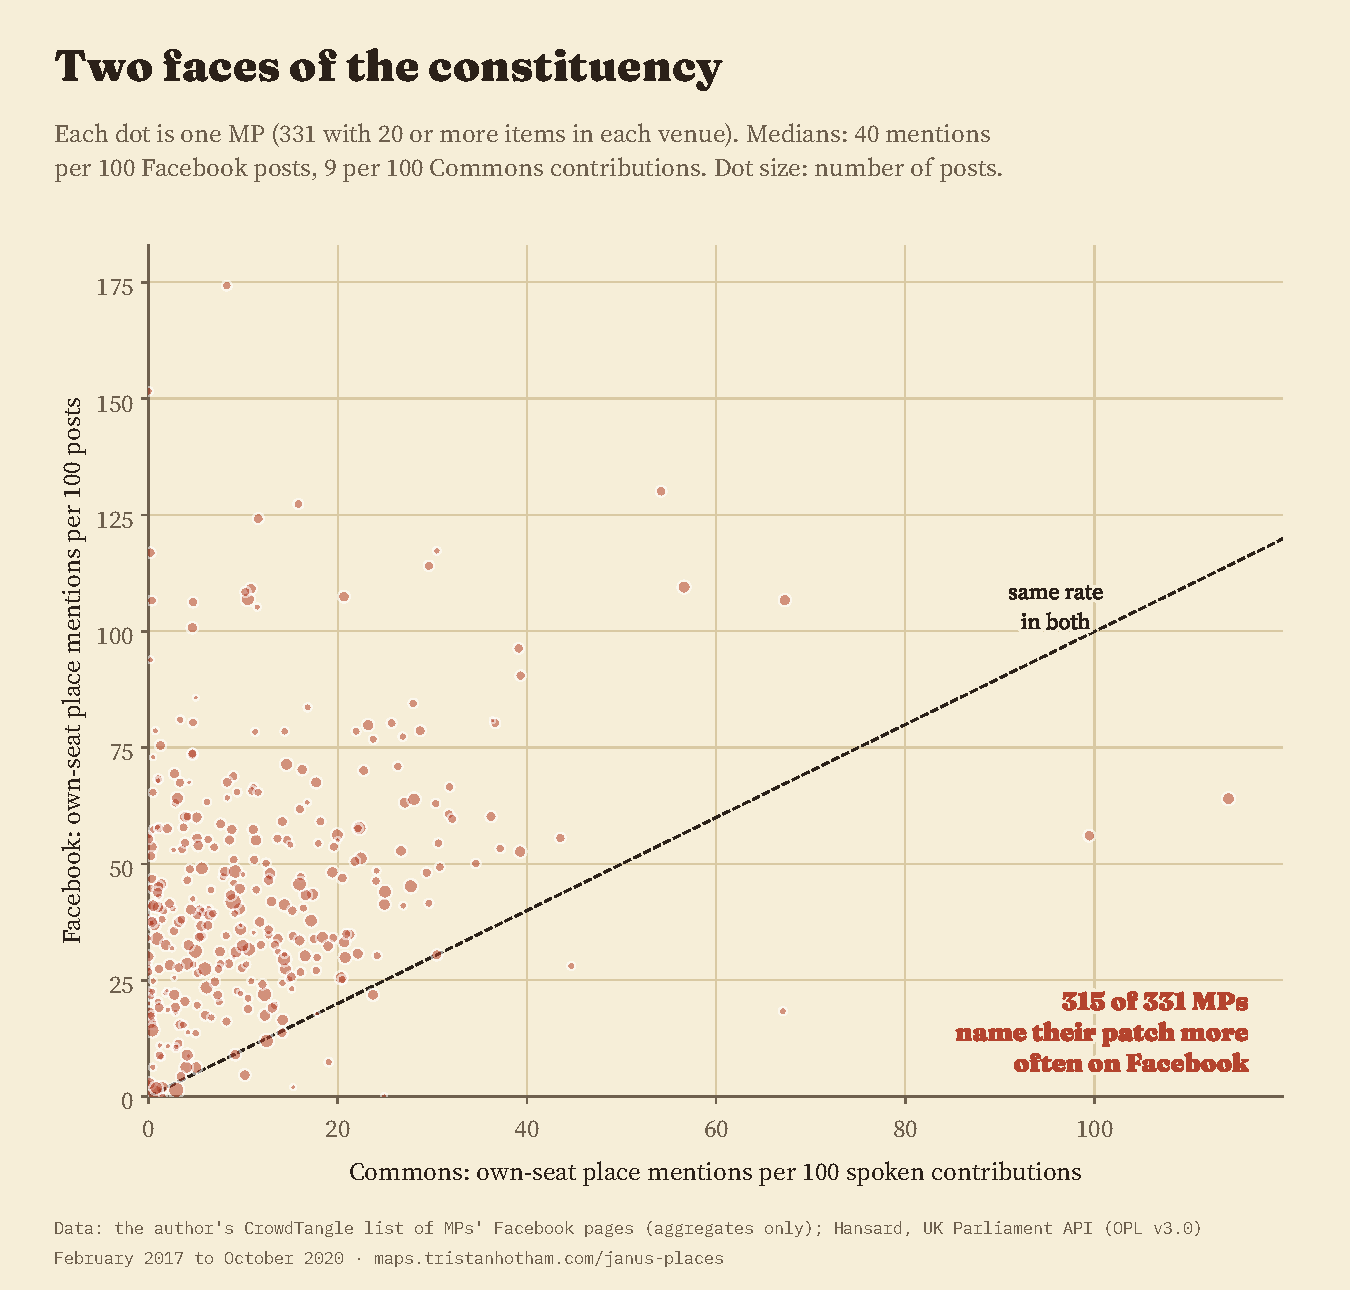
\includegraphics[width=0.82\textwidth]{f_scatter.pdf}
\caption{Each MP's own-seat place mentions per 100 Facebook posts against per 100 spoken Commons contributions, February 2017 to October 2020. MPs with at least 20 items in each venue. The dashed line marks equal rates.}\label{fig:scatter}
\end{figure}

\begin{table}[tbp]\centering\small\caption{Own-seat place mentions per 100 items in each venue, and the within-MP Facebook to Commons rate ratio (PPML with spell and month fixed effects, offset log items, standard errors clustered by spell; 95\% CI). N = 22,979 spell-venue-months, 358 spells.}\label{tab:main}\begin{tabular}{lrrlr}\toprule Places & Facebook & Commons & Rate ratio [95\% CI] & $p$\\\midrule
Main place set & 42.33 & 9.00 & 4.36 [3.76, 5.06] & $<$0.001\\
Places in the seat's name & 23.79 & 5.74 & 3.54 [3.10, 4.03] & $<$0.001\\
Most populous other places & 12.86 & 2.23 & 6.06 [4.93, 7.46] & $<$0.001\\
Random sample of other places (weighted) & 5.68 & 1.03 & 5.55 [3.20, 9.62] & $<$0.001\\
Placebo: places in another seat & 0.02 & 0.03 & 1.04 [0.65, 1.66] & 0.867\\
\bottomrule\end{tabular}\end{table}

The gap is present in every month in which both venues are active (Figure~\ref{fig:monthly}): the Facebook rate was higher in 40 of 40 such months. The Facebook rate ranged from about 27 to 68 mentions per 100 posts and the Commons rate from about 5 to 21 per 100 contributions. During election campaigns, when Parliament does not sit, 41\% of MPs' posts with a message named at least one place in their seat, against 32\% in sitting months.

\begin{figure}[tbp]\centering
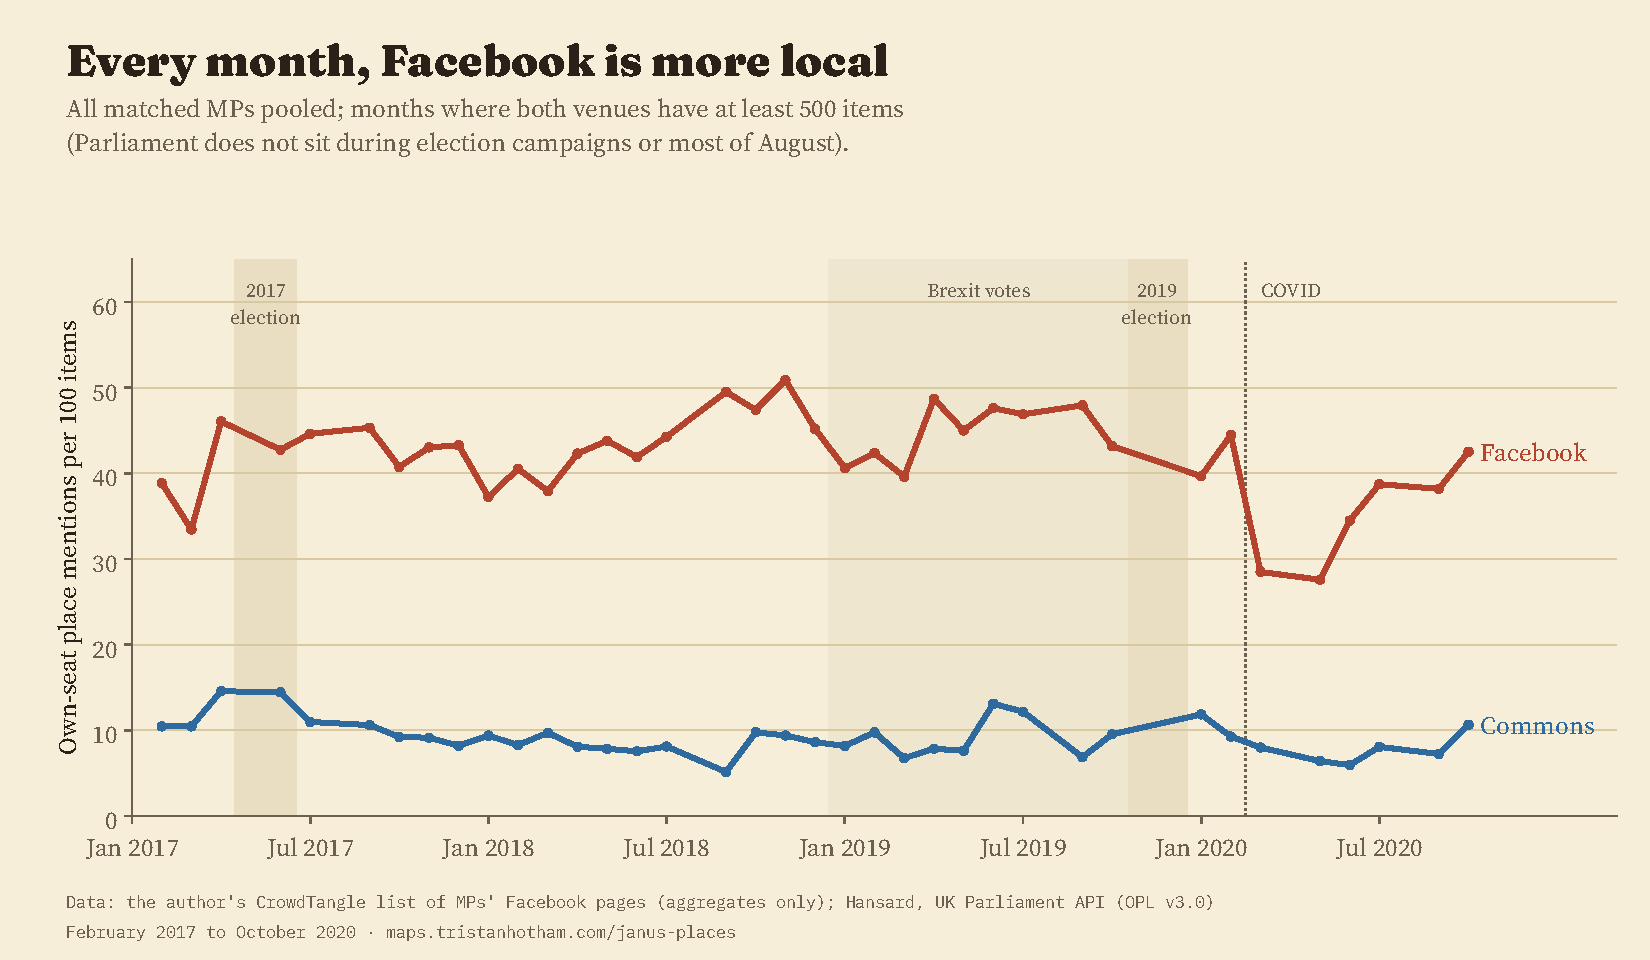
\includegraphics[width=\textwidth]{f_monthly.pdf}
\caption{Own-seat place mentions per 100 items by month, all matched MPs pooled, for months with at least 500 items in both venues.}\label{fig:monthly}
\end{figure}

\subsection{Which places}
The gap does not depend on the kind of place (Figure~\ref{fig:groups}). For the places in the seat's own name, the Facebook rate is 23.8 and the Commons rate 5.7 per 100 items (within-MP rate ratio 3.5). For the other places, the most populous ones and the weighted random sample, it is 18.5 against 3.3 (rate ratio 5.9). The seat's name carries a larger share of local naming in the Commons, which fits a chamber in which MPs speak of ``my constituency of'' the seat, while Facebook spreads more of its local naming across the other places.

\begin{figure}[tbp]\centering
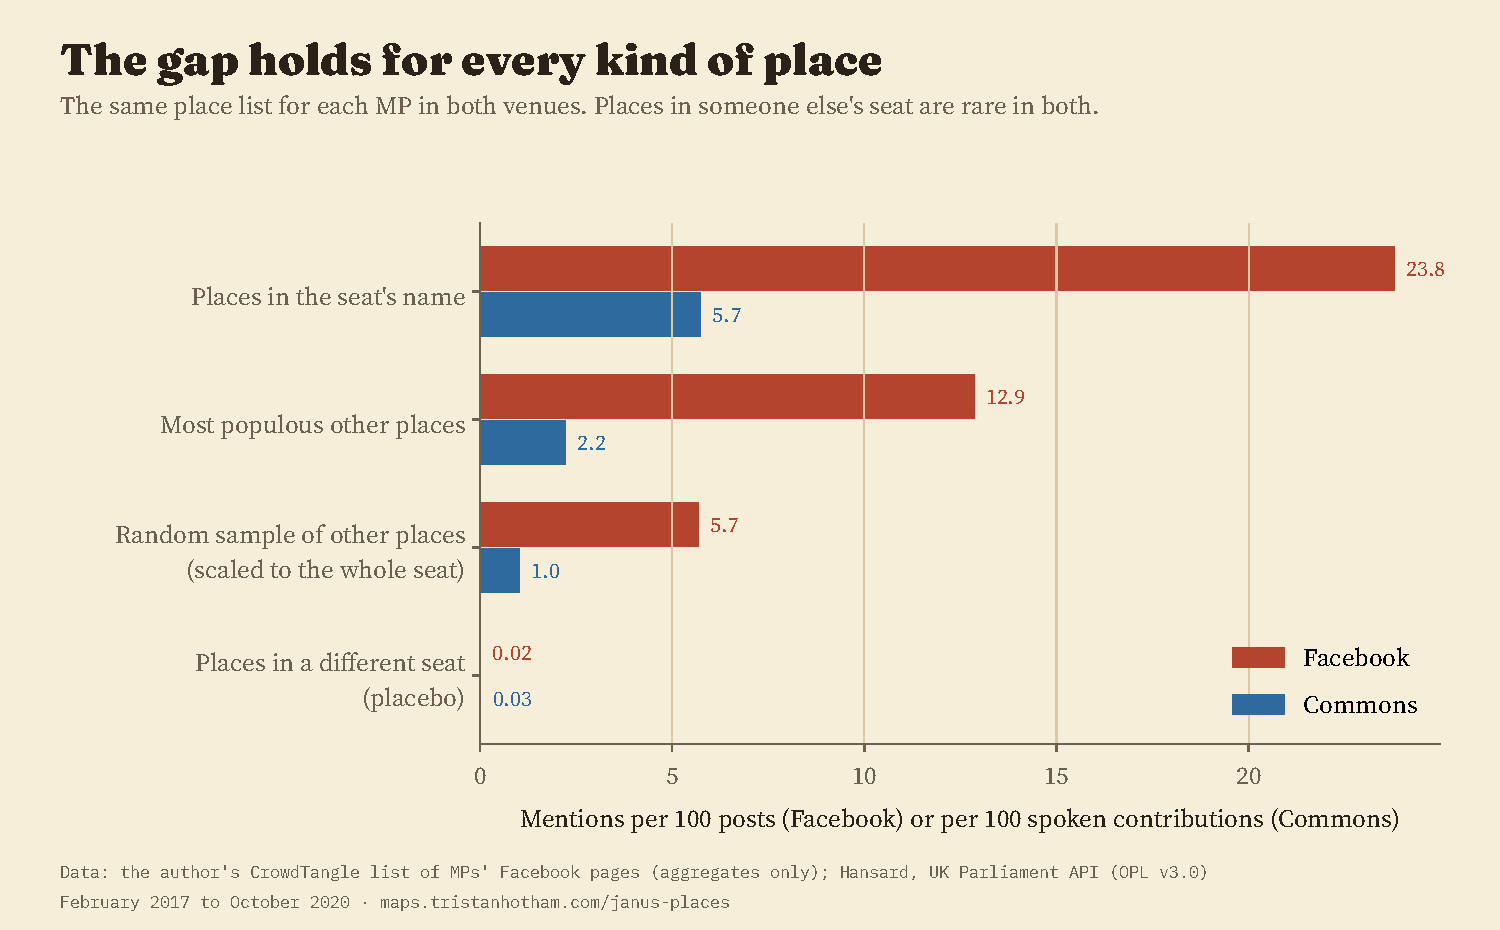
\includegraphics[width=0.9\textwidth]{f_groups.pdf}
\caption{Mentions per 100 items by group of place, all matched MPs, pooled over the window. Random sample places are weighted to the whole seat. Placebo places lie in a different seat.}\label{fig:groups}
\end{figure}

H2 expected Facebook to reach further down the settlement hierarchy, naming small places relatively more often. It does not, in the planned test (Figure~\ref{fig:size}). The population elasticity of naming is 1.01 in the Commons (95\% CI 0.84 to 1.17) and 0.95 on Facebook; the difference, -0.06 (CI -0.21 to 0.09; 2,598 places in 352 spells), cannot be told apart from zero. Facebook names places of every size more often, by a similar factor. The other two planned measures point in the same direction, with small differences. Among 280 MPs with at least five local mentions in each venue, the largest place in the seat took 37\% of local naming on Facebook and 41\% in the Commons. And because Facebook names places so much more often, the weighted share of an MP's non-seat-name places named at least once was 40\% on Facebook against 16\% in the Commons; this measure rises with volume and is not a test of breadth on its own. H2 is not supported: the local face is louder, not differently shaped.

\begin{figure}[tbp]\centering
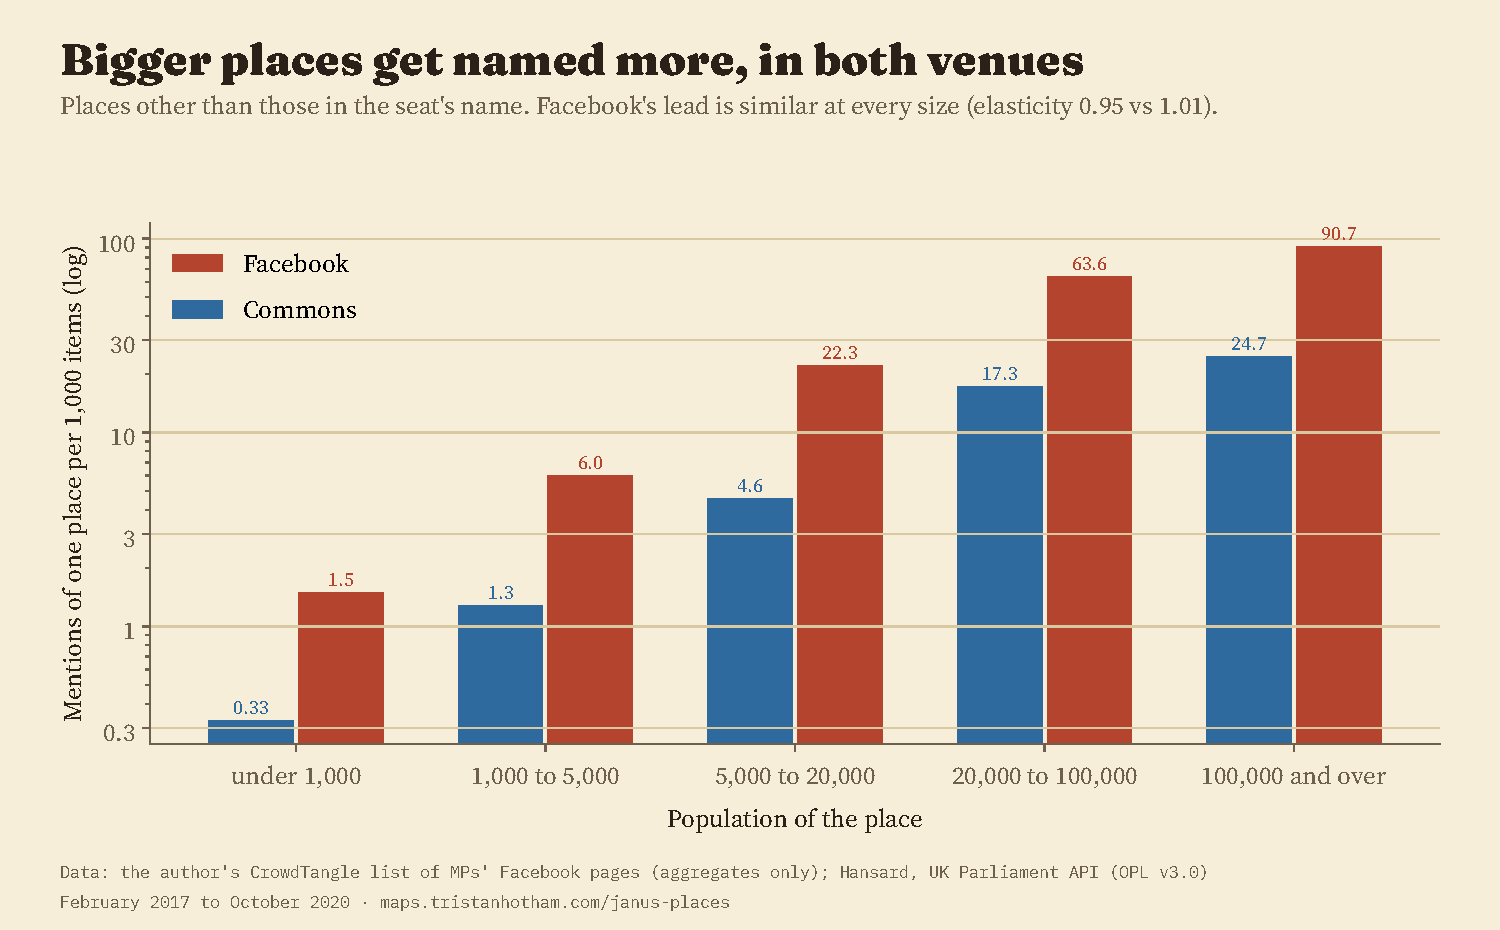
\includegraphics[width=0.9\textwidth]{f_size.pdf}
\caption{Mentions of a single place per 1,000 items, by the place's population, for places other than those in the seat's name (most populous and weighted random sample). Log scale.}\label{fig:size}
\end{figure}

\subsection{Who and when}
Table~\ref{tab:het} and Figure~\ref{fig:who} report the planned interactions. Marginality works the opposite way to H3. In spells and months where the seat's majority was under ten points, the Facebook to Commons ratio was 33\% smaller than elsewhere (ratio of rate ratios 0.67, CI 0.49 to 0.91; 142 spells had a marginal majority at some point); for each ten points of majority, the ratio was 10\% larger (CI 1.00 to 1.22, $p$ = 0.05). MPs in marginal seats were, if anything, more local in the Commons relative to their pages. H3 is not supported.

The gap varies with office, but not in the direction I expected. In months when an MP held a frontbench post, the Facebook to Commons ratio was 2.7 times as large (CI 2.0 to 3.8; 226 spells held such a post at some point), so H4, which expected a smaller gap, is not supported. Separate models for each venue (added after the plan) show where the difference lies. Within MP, the Commons rate in frontbench months was 77\% lower than in the same MP's other months (CI 69\% to 83\%), while the Facebook rate did not change (rate ratio 1.00, CI 0.92 to 1.09). In frontbench months, the Commons contributions name the constituency less, while the Facebook page names it as often as before. Including whips in the frontbench measure gives a similar result (2.6). MPs on the government side also had a larger gap (2.3 times, CI 1.7 to 3.0), and both differences remain when they are estimated together (exploratory: frontbench 2.8, government side 2.3). Government-side membership barely changes within a spell, so this is a comparison between MPs, and it may reflect the different uses that government and opposition backbenchers make of the chamber; I do not compare parties further.

\begin{figure}[tbp]\centering
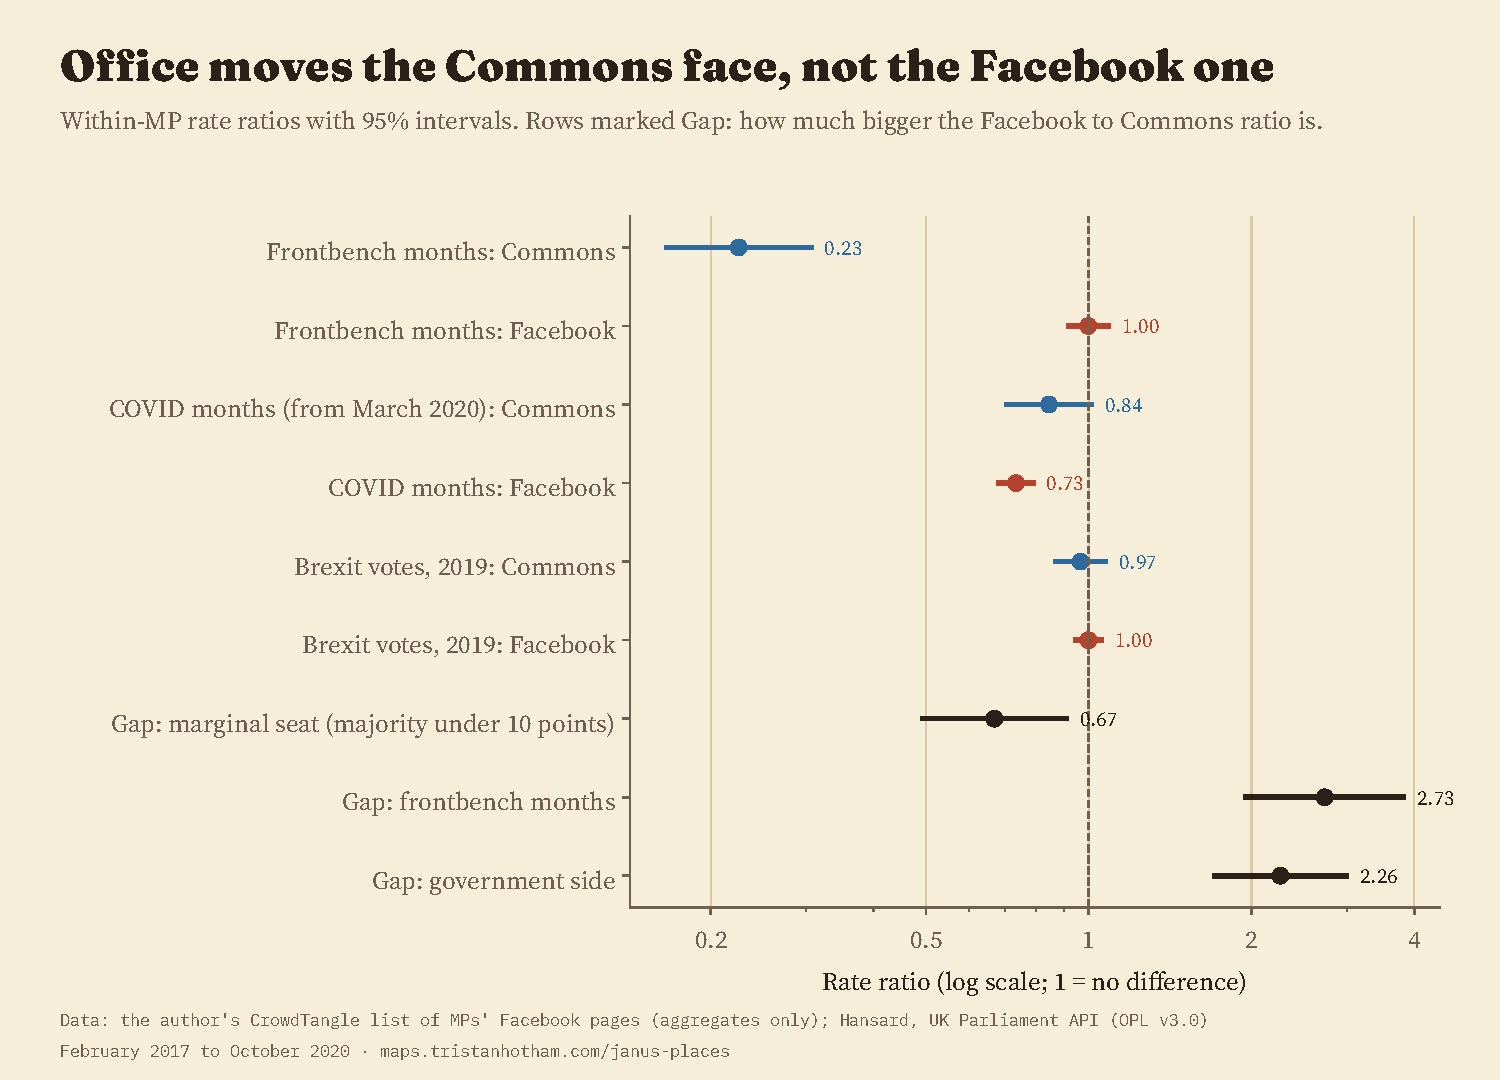
\includegraphics[width=0.92\textwidth]{f_who.pdf}
\caption{Within-MP rate ratios with 95\% confidence intervals. Rows naming a venue compare the period with the same MP's other months in that venue. Rows marked ``Gap'' are ratios of the Facebook to Commons rate ratio.}\label{fig:who}
\end{figure}

\begin{table}[tbp]\centering\footnotesize\caption{Planned tests of H2 to H5. H2 rows are coefficients on log population (PPML, spell-by-venue fixed effects, random-sample weights). Rows marked gap are ratios of the Facebook to Commons rate ratio; venue-only rows compare the period with the same MP's other months. Standard errors clustered by spell.}\label{tab:het}\begin{tabular}{p{7.2cm}lrr}\toprule Term & Estimate [95\% CI] & Unit & N\\\midrule
H2: population elasticity, Commons & 1.01 [0.84, 1.17] & place-venue & 4,487\\
H2: Facebook minus Commons elasticity & -0.06 [-0.21, 0.09] & place-venue & 4,487\\
H3: gap $\times$ majority (per 10 points) & 1.10 [1.00, 1.22] & month & 22,979\\
H3: gap $\times$ marginal ($<$10 points) & 0.67 [0.49, 0.91] & month & 22,979\\
H4: gap $\times$ frontbench & 2.73 [1.96, 3.81] & month & 22,979\\
H4: gap $\times$ frontbench incl. whips & 2.55 [1.86, 3.50] & month & 22,979\\
H4: gap $\times$ government side & 2.26 [1.71, 2.99] & month & 22,979\\
H4 (exploratory): frontbench, Commons only & 0.23 [0.17, 0.31] & month & 10,055\\
H4 (exploratory): frontbench, Facebook only & 1.00 [0.92, 1.09] & month & 12,729\\
H4 (exploratory): joint, frontbench & 2.85 [2.12, 3.83] & month & 22,979\\
H4 (exploratory): joint, government side & 2.32 [1.80, 3.00] & month & 22,979\\
H5 (exploratory): gap $\times$ Brexit months & 1.07 [0.94, 1.22] & month & 22,979\\
H5 (exploratory): Brexit months, Facebook only & 1.00 [0.95, 1.05] & month & 12,729\\
H5 (exploratory): Brexit months, Commons only & 0.97 [0.87, 1.07] & month & 10,055\\
H5 (exploratory): gap $\times$ COVID months & 0.94 [0.75, 1.17] & month & 22,979\\
H5 (exploratory): COVID months, Facebook only & 0.73 [0.68, 0.79] & month & 12,729\\
H5 (exploratory): COVID months, Commons only & 0.84 [0.71, 1.01] & month & 10,055\\
H5 (exploratory): gap $\times$ two months before an election was called & 0.91 [0.78, 1.07] & month & 22,979\\
H5 (exploratory): two months before an election was called, Facebook only & 1.00 [0.95, 1.06] & month & 12,729\\
H5 (exploratory): two months before an election was called, Commons only & 1.08 [0.97, 1.21] & month & 10,055\\
\bottomrule\end{tabular}\end{table}

The time patterns (H5, exploratory) are modest. In the Brexit months of 2019 neither venue's local rate changed (Facebook 1.00, Commons 0.97). From March 2020, the Facebook rate fell by 27\% (CI 0.68 to 0.79), and recovered over the summer (Figure~\ref{fig:monthly}); the Commons rate fell by 16\%, with an interval that includes no change. In the two sitting months before each election was called, neither venue changed clearly. None of these period interactions changes the size of the gap clearly.

\section{Placebo and robustness}\label{sec:robust}
Places in another MP's seat are a placebo: if the gap reflected nothing more than Facebook's habit of naming places, it would appear for them too. It does not. Placebo places were named 0.023 times per 100 posts and 0.025 times per 100 contributions, a rate ratio of 1.04 (CI 0.65 to 1.66). The excess on Facebook is specific to the MP's own seat.

Figure~\ref{fig:robust} and Table~\ref{tab:robust} report the 15 planned and added checks: counting any Facebook text field, dropping ambiguous names, dropping or keeping only seat-name places, the most populous places only, the random sample only, MP-quarters instead of months, MPs with at least 20 items in each venue, leaving out each nation, dropping the ten largest pages, dropping Deputy Speakers (added after the plan, because their Commons contributions are mostly from the chair), and a negative binomial model. The rate ratio ranges from 3.1 to 6.1, and its confidence interval excludes 1 in all 15. It is smallest when England is left out (3.1) and when only seat-name places are counted (3.5), and largest for the most populous other places (6.1).

\begin{figure}[tbp]\centering
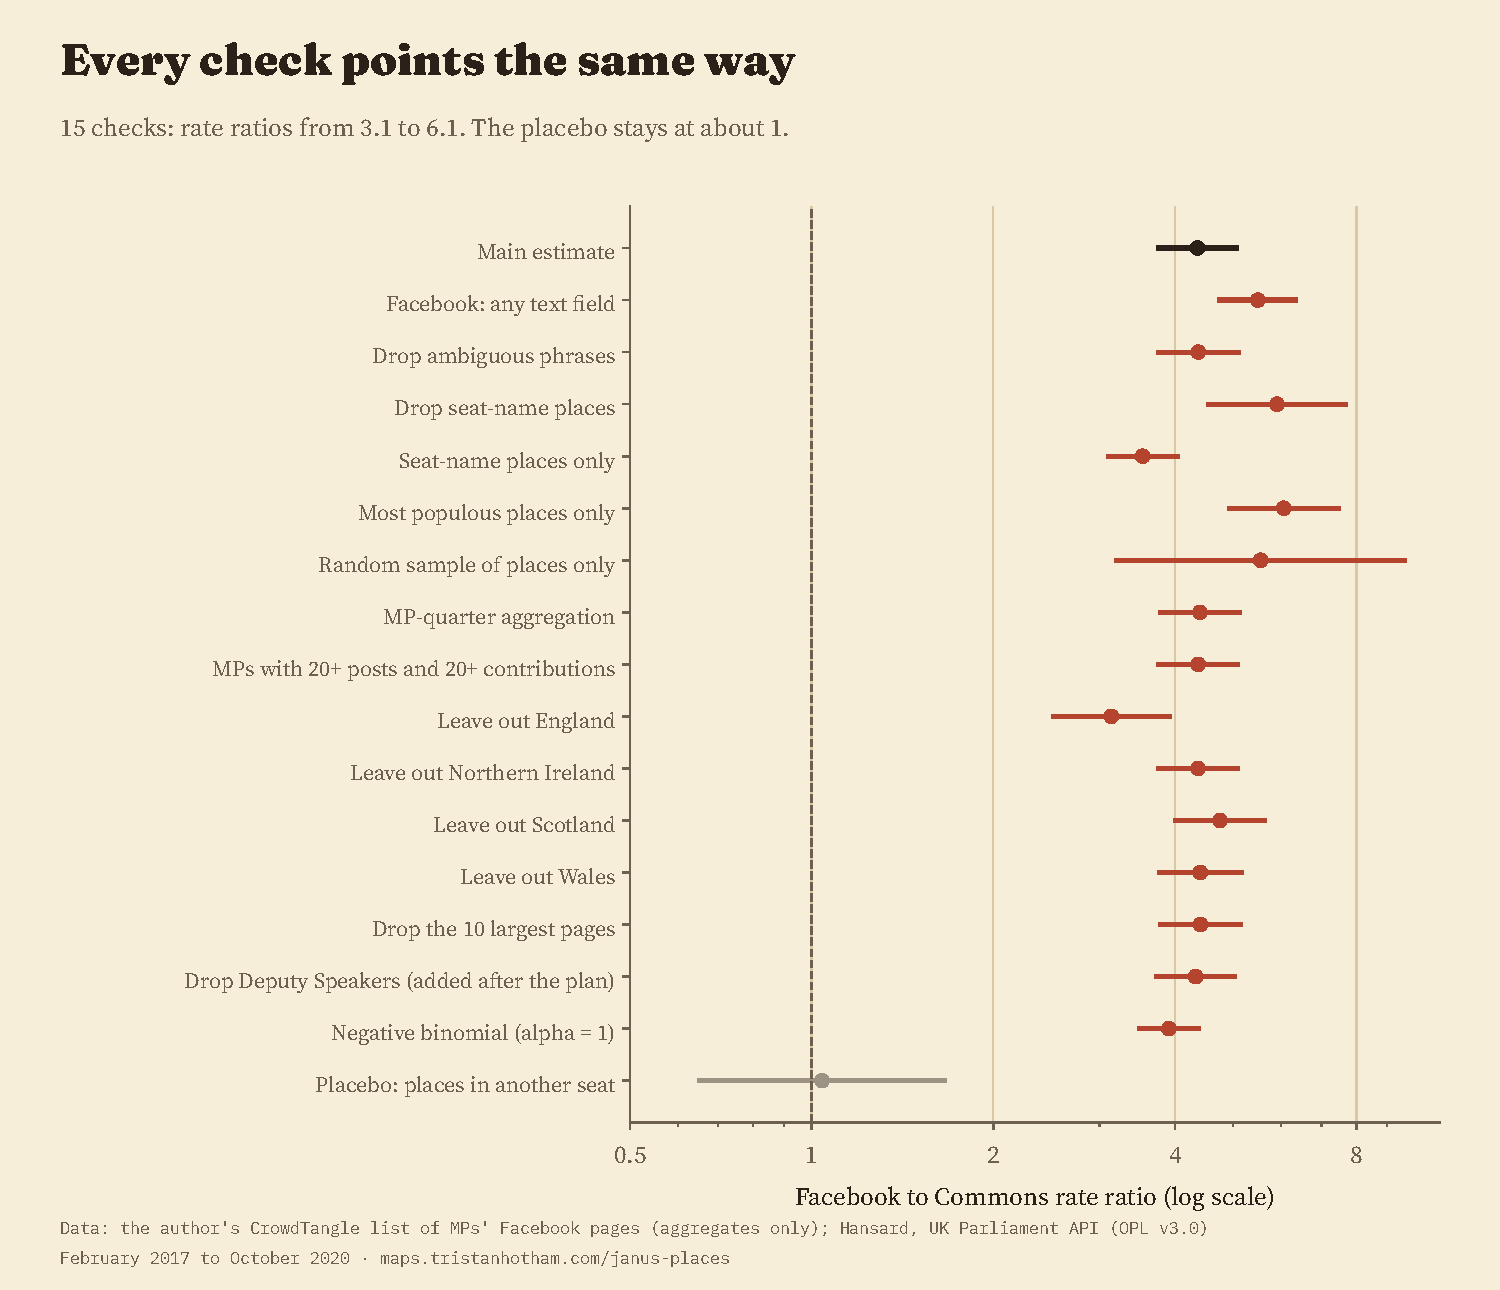
\includegraphics[width=0.92\textwidth]{f_robust.pdf}
\caption{The Facebook to Commons rate ratio in each check, with 95\% confidence intervals, and the placebo.}\label{fig:robust}
\end{figure}

\begin{table}[tbp]\centering\small\caption{Robustness: the Facebook to Commons rate ratio under each check (95\% CI).}\label{tab:robust}\begin{tabular}{lrrr}\toprule Check & Rate ratio [95\% CI] & N & Spells\\\midrule
Main estimate & 4.36 [3.76, 5.06] & 22,979 & 358\\\midrule
Facebook: any text field & 5.49 [4.75, 6.35] & 22,979 & 358\\
Drop ambiguous phrases & 4.37 [3.76, 5.09] & 22,972 & 358\\
Drop seat-name places & 5.91 [4.55, 7.67] & 22,801 & 358\\
Seat-name places only & 3.54 [3.10, 4.03] & 20,462 & 358\\
Most populous places only & 6.06 [4.93, 7.46] & 22,173 & 358\\
Random sample of places only & 5.55 [3.20, 9.62] & 18,478 & 358\\
MP-quarter aggregation & 4.40 [3.79, 5.11] & 9,484 & 358\\
MPs with 20+ posts and 20+ contributions & 4.37 [3.76, 5.08] & 22,604 & 331\\
Leave out England & 3.14 [2.51, 3.92] & 4,552 & 75\\
Leave out Northern Ireland & 4.37 [3.76, 5.08] & 22,657 & 352\\
Leave out Scotland & 4.75 [4.02, 5.62] & 19,954 & 307\\
Leave out Wales & 4.41 [3.77, 5.15] & 21,774 & 340\\
Drop the 10 largest pages & 4.41 [3.79, 5.13] & 22,288 & 348\\
Drop Deputy Speakers (added after the plan) & 4.33 [3.73, 5.03] & 22,898 & 357\\
Negative binomial (alpha = 1) & 3.91 [3.50, 4.37] & 22,979 & 358\\
\bottomrule\end{tabular}\end{table}

Figure~\ref{fig:map} maps the gap by seat. It is widespread: in 326 of the 350 seats with a matched MP the Facebook rate is higher, and the exceptions are scattered.

\begin{figure}[tbp]\centering
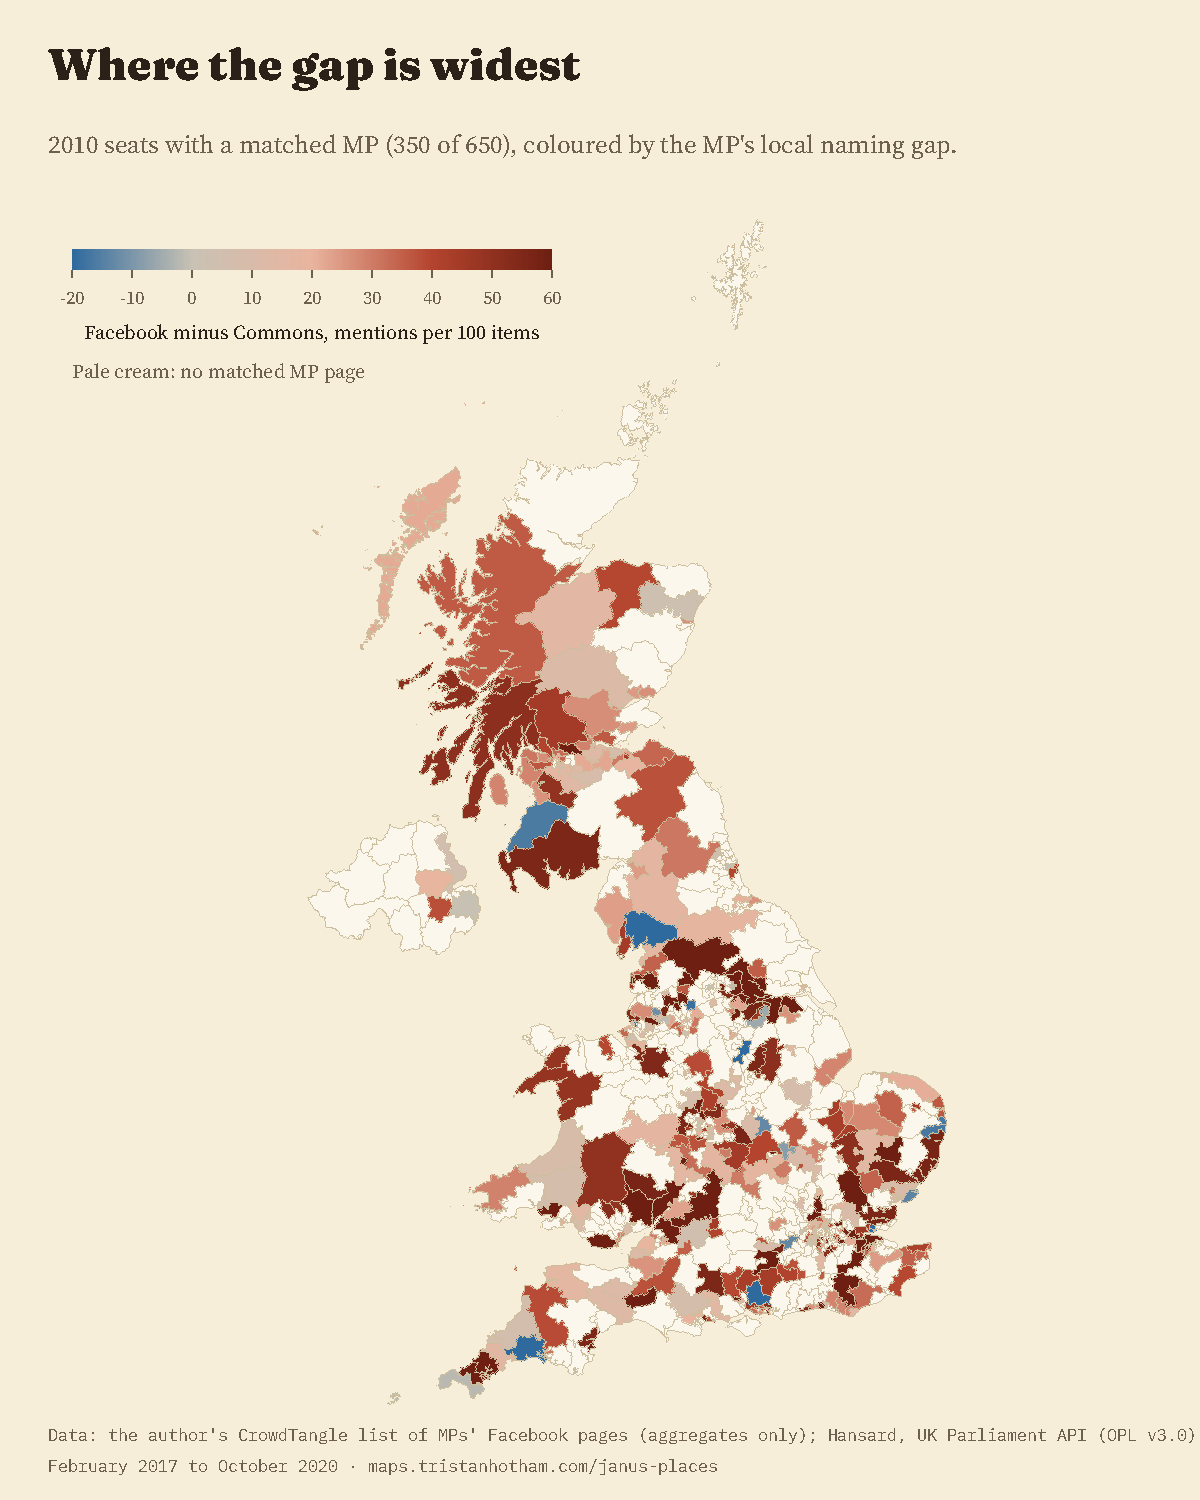
\includegraphics[width=0.72\textwidth]{f_map.pdf}
\caption{Each 2010 constituency with a matched MP, coloured by the MP's Facebook rate minus Commons rate (own-seat place mentions per 100 items); where a seat had two matched MPs in the window, the one with more posts is shown.}\label{fig:map}
\end{figure}

\section{Discussion}\label{sec:disc}
\subsection{What the pattern says}
British MPs present two faces of their constituency. On Facebook they name the towns and villages they represent about four to five times as often, per item, as they do in their spoken contributions in the House of Commons. The gap is not an artefact of Facebook naming places in general, because places in other seats are named equally rarely in both venues, and it is not a matter of a few town names, because it holds for villages and for the random sample of places. Nor is the local face differently shaped: both venues name bigger places more, at much the same rate, so the Facebook page is a louder version of the same map rather than a different map.

A second result is about office. In months when an MP is on the front bench her Commons contributions name her seat's places far less often, while her Facebook page keeps the same local rate. In the terms of home style, the Washington face changes with the job and the home face does not. This complements the finding, in a working paper on the same archive, that frontbench MPs' pages were less local than backbenchers' \citep{hotham2027}: comparing the same MP before and during office, it is the Commons voice that changes, not the page. It also qualifies the use of parliamentary speech as a measure of constituency focus: a frontbencher's low rate of local naming in the chamber is a feature of the role, and her constituency may be no less present in what she says to it directly.

The marginality result runs against a common expectation in the constituency focus literature \citep{kellermann2016,andre2015}. If MPs in marginal seats work harder to be seen to serve the constituency, the evidence here suggests that they do so at least as much in the chamber as on their pages: the gap between the two faces is smaller in marginal seats. One reading is that the Commons is itself a stage for constituency signals, through questions, adjournment debates and mentions in speeches, and that MPs with most to lose use it. Another is that the seats in this sample that were marginal differ in other ways. The design cannot separate these readings.

\subsection{Limitations}
The Facebook data set the window: because the export reached CrowdTangle's row cap, nothing before 11 February 2017 is available, and the analysis covers only February 2017 to October 2020, a period with two general elections, the Brexit votes and the start of COVID. The list of pages is one researcher's selection, made for doctoral research, and over-represents MPs who were active on Facebook; only 350 of the 650 seats have a matched MP with items in both venues. Counts measure naming, not meaning: a post can name a town to celebrate it or to criticise a decision, and the measure does not distinguish. The rate is per item, and posts and contributions differ in length and function. The place lists rest on Wikidata's settlements and on simplified boundaries, and some names remain ambiguous despite the flags; the checks without ambiguous names and without seat-name places give similar results. Hansard's search counts contributions containing a phrase, and it cannot tell who else a contribution refers to. Finally, the design is observational. It shows where MPs name the places they represent, not why, and none of the associations with office, marginality or side should be read as causal effects.

\subsection{Implications}
For research on representation, the results suggest that measures of constituency focus based on parliamentary text capture only part of how MPs present their constituency, and that the part they capture changes with office. Comparisons of MPs' constituency focus that rely on speeches or questions will understate it for frontbenchers. For research on political communication, they show that MPs' pages were, in this period, local media: about a third of posts with a message named at least one place in the MP's seat. The method, a fixed place list searched with the same rule in two venues, can be repeated wherever speeches can be searched by member and phrase and wherever social media archives exist.

\section{Conclusion}\label{sec:conc}
For the same MP, in the same months and for the same places, the constituency is about four times as visible on Facebook as in the House of Commons. The gap is general, it is specific to the MP's own seat, and it is wider in months when an MP holds frontbench office, when her Commons contributions name her seat less often while her page does not change. These are two faces of one representative, and studies that look at only one of them see only half of how British MPs represent their places.

\section*{Data availability statement}
Data and code: Zenodo DOI https://doi.org/10.5281/zenodo.24105795. The archive contains the place lists, the query list, the Hansard monthly counts, the Facebook counts per MP, month and place, the MP-page matches and all code. Facebook post text, links and URLs are not shared, in line with CrowdTangle's terms; only aggregate counts are.

\section*{AI statement}
I wrote the text, with drafting and editing assistance from Claude (Anthropic), which also helped prepare the analysis code. I reviewed and checked all text and results.

\begin{thebibliography}{99}
\bibitem[Abadie et al.(2023)]{abadie2023} Abadie, A., Athey, S., Imbens, G. W. and Wooldridge, J. M. (2023) When should you adjust standard errors for clustering? \textit{Quarterly Journal of Economics} 138(1), 1 to 35. doi:10.1093/qje/qjac038.
\bibitem[Andr\'e et al.(2015)]{andre2015} Andr\'e, A., Depauw, S. and Martin, S. (2015) Electoral systems and legislators' constituency effort: the mediating effect of electoral vulnerability. \textit{Comparative Political Studies} 48(4), 464 to 496. doi:10.1177/0010414014545512.
\bibitem[Bright et al.(2020)]{bright2020} Bright, J., Hale, S., Ganesh, B., Bulovsky, A., Margetts, H. and Howard, P. (2020) Does campaigning on social media make a difference? Evidence from candidate use of Twitter during the 2015 and 2017 U.K. elections. \textit{Communication Research} 47(7), 988 to 1009. doi:10.1177/0093650219872394.
\bibitem[Cain et al.(1987)]{cain1987} Cain, B., Ferejohn, J. and Fiorina, M. (1987) \textit{The Personal Vote: Constituency Service and Electoral Independence}. Cambridge, MA: Harvard University Press. doi:10.4159/harvard.9780674493285.
\bibitem[Cameron and Miller(2015)]{cameron2015} Cameron, A. C. and Miller, D. L. (2015) A practitioner's guide to cluster-robust inference. \textit{Journal of Human Resources} 50(2), 317 to 372.
\bibitem[Campbell and Lovenduski(2015)]{campbell2015} Campbell, R. and Lovenduski, J. (2015) What should MPs do? Public and parliamentarians' views compared. \textit{Parliamentary Affairs} 68(4), 690 to 708.
\bibitem[Correia et al.(2020)]{correia2020} Correia, S., Guimar\~aes, P. and Zylkin, T. (2020) Fast Poisson estimation with high-dimensional fixed effects. \textit{Stata Journal} 20(1), 95 to 115. doi:10.1177/1536867X20909691.
\bibitem[CrowdTangle Team(2020)]{crowdtangle2020} CrowdTangle Team (2020) \textit{CrowdTangle}. Facebook, Menlo Park, CA. List of UK MPs' pages, historical export October 2020.
\bibitem[Enli and Skogerb\o(2013)]{enli2013} Enli, G. S. and Skogerb\o, E. (2013) Personalized campaigns in party-centred politics: Twitter and Facebook as arenas for political communication. \textit{Information, Communication \& Society} 16(5), 757 to 774. doi:10.1080/1369118X.2013.782330.
\bibitem[Eulau and Karps(1977)]{eulau1977} Eulau, H. and Karps, P. D. (1977) The puzzle of representation: specifying components of responsiveness. \textit{Legislative Studies Quarterly} 2(3), 233 to 254. doi:10.2307/439340.
\bibitem[Fenno(1978)]{fenno1978} Fenno, R. F. (1978) \textit{Home Style: House Members in Their Districts}. Boston: Little, Brown.
\bibitem[Fernandes et al.(2018)]{fernandes2018} Fernandes, J. M., Leston-Bandeira, C. and Schwemmer, C. (2018) Election proximity and representation focus in party-constrained environments. \textit{Party Politics} 24(6), 674 to 685. doi:10.1177/1354068817689955.
\bibitem[Grimmer(2013)]{grimmer2013} Grimmer, J. (2013) \textit{Representational Style in Congress: What Legislators Say and Why It Matters}. Cambridge: Cambridge University Press.
\bibitem[Hansard(2026)]{hansard2026} UK Parliament (2026) Hansard API, search and timeline statistics for House of Commons spoken contributions. Retrieved 2026. Open Parliament Licence v3.0.
\bibitem[Hotham(2021)]{hotham2021} Hotham, T. (2021) \textit{How Do Political Parties Use Facebook and What Does It Offer to Their Campaigns?} PhD thesis, University of Bath.
\bibitem[Hotham(2026a)]{hotham2026a} Hotham, T. (2026a) \textit{Mentioned in the House: which places does Parliament talk about? Place mentions in House of Commons debates, 1909 to 2026}. Zenodo. doi:10.5281/zenodo.23761431.
\bibitem[Hotham(2026b)]{hotham2026b} Hotham, T. (2026b) \textit{Who Won Here? UK general election results by constituency, 1832 to 2024}. Zenodo. doi:10.5281/zenodo.23761425.
\bibitem[Hotham(2026c)]{hotham2026c} Hotham, T. (2026c) \textit{Do by-elections make Parliament listen? Parliamentary attention to by-election constituencies in the House of Commons, 1911 to 2023}. Preprint, Zenodo. doi:10.5281/zenodo.24094210.
\bibitem[Hotham(2027)]{hotham2027} Hotham, T. (2027) Ahead of the tide? British MPs' Facebook pages and their results against their party's swing, 2017 and 2019. Working paper.
\bibitem[Jackson and Lilleker(2011)]{jackson2011} Jackson, N. and Lilleker, D. (2011) Microblogging, constituency service and impression management: UK MPs and the use of Twitter. \textit{Journal of Legislative Studies} 17(1), 86 to 105. doi:10.1080/13572334.2011.545181.
\bibitem[Kellermann(2016)]{kellermann2016} Kellermann, M. (2016) Electoral vulnerability, constituency focus, and parliamentary questions in the House of Commons. \textit{British Journal of Politics and International Relations} 18(1), 90 to 106.
\bibitem[Mansbridge(2003)]{mansbridge2003} Mansbridge, J. (2003) Rethinking representation. \textit{American Political Science Review} 97(4), 515 to 528.
\bibitem[Martin(2011)]{martin2011} Martin, S. (2011) Using parliamentary questions to measure constituency focus: an application to the Irish case. \textit{Political Studies} 59(2), 472 to 488.
\bibitem[mySociety(2026)]{parlparse2026} mySociety (2026) parlparse: members data (people.json, ministers-2010.json). GitHub, github.com/mysociety/parlparse, retrieved 2026. Records of the House of Commons, Open Parliament Licence v3.0.
\bibitem[Norton(1994)]{norton1994} Norton, P. (1994) The growth of the constituency role of the MP. \textit{Parliamentary Affairs} 47(4), 705 to 720.
\bibitem[Norton and Wood(1993)]{norton1993} Norton, P. and Wood, D. M. (1993) \textit{Back from Westminster: British Members of Parliament and Their Constituents}. Lexington: University Press of Kentucky.
\bibitem[Proksch and Slapin(2015)]{proksch2015} Proksch, S.-O. and Slapin, J. B. (2015) \textit{The Politics of Parliamentary Debate: Parties, Rebels and Representation}. Cambridge: Cambridge University Press.
\bibitem[Russo(2011)]{russo2011} Russo, F. (2011) The constituency as a focus of representation: studying the Italian case through the analysis of parliamentary questions. \textit{Journal of Legislative Studies} 17(3), 290 to 301. doi:10.1080/13572334.2011.595122.
\bibitem[Santos Silva and Tenreyro(2006)]{santos2006} Santos Silva, J. M. C. and Tenreyro, S. (2006) The log of gravity. \textit{Review of Economics and Statistics} 88(4), 641 to 658. doi:10.1162/rest.88.4.641.
\bibitem[Searing(1985)]{searing1985} Searing, D. D. (1985) The role of the good constituency member and the practice of representation in Great Britain. \textit{Journal of Politics} 47(2), 348 to 381.
\bibitem[Searing(1994)]{searing1994} Searing, D. D. (1994) \textit{Westminster's World: Understanding Political Roles}. Cambridge, MA: Harvard University Press.
\bibitem[Soroka et al.(2009)]{soroka2009} Soroka, S., Penner, E. and Blidook, K. (2009) Constituency influence in Parliament. \textit{Canadian Journal of Political Science} 42(3), 563 to 591.
\bibitem[Southern and Lee(2019)]{southern2019} Southern, R. and Lee, B. (2019) Politics as usual? Assessing the extent and content of candidate-level online campaigning at the 2015 UK general election. \textit{Journal of Elections, Public Opinion and Parties} 29(2), 179 to 198. doi:10.1080/17457289.2018.1515209.
\bibitem[Stier et al.(2018)]{stier2018} Stier, S., Bleier, A., Lietz, H. and Strohmaier, M. (2018) Election campaigning on social media: politicians, audiences, and the mediation of political communication on Facebook and Twitter. \textit{Political Communication} 35(1), 50 to 74. doi:10.1080/10584609.2017.1334728.
\bibitem[UK-GeoJSON(2026)]{ukgeojson} Chorley, M. J. (2026) UK-GeoJSON: Northern Ireland Westminster parliamentary constituencies (json/electoral/ni/wpc.json). GitHub, github.com/martinjc/UK-GeoJSON, retrieved 2026. Contains public sector information licensed under the Open Government Licence v3.0.
\bibitem[Vivyan and Wagner(2016)]{vivyan2016} Vivyan, N. and Wagner, M. (2016) House or home? Constituent preferences over legislator effort allocation. \textit{European Journal of Political Research} 55(1), 81 to 99. doi:10.1111/1475-6765.12119.
\bibitem[Wikidata(2026)]{wikidata2026} Wikidata contributors (2026) UK human settlements with coordinates and population. Retrieved 2026 through QLever. CC0.
\bibitem[Zittel et al.(2019)]{zittel2019} Zittel, T., Nyhuis, D. and Baumann, M. (2019) Geographic representation in party-dominated legislatures: a quantitative text analysis of parliamentary questions in the German Bundestag. \textit{Legislative Studies Quarterly} 44(4), 681 to 711. doi:10.1111/lsq.12238.
\end{thebibliography}

\appendix
\section{Appendix: full tables and data construction}
\begin{table}[htbp]\centering\small\caption{Median own-seat place mentions per 100 items by nation, MPs with at least 20 items in each venue (descriptive).}\label{tab:appx}\begin{tabular}{lrrr}\toprule Nation & MPs & Facebook & Commons\\\midrule
England & 261 & 41.2 & 8.9\\
Northern Ireland & 6 & 19.8 & 4.7\\
Scotland & 47 & 34.2 & 10.0\\
Wales & 17 & 53.9 & 8.8\\
\bottomrule\end{tabular}\end{table}

Table~\ref{tab:appx} gives the median rates by nation. \textbf{Decisions made by hand.} Sixteen pages were matched by hand to members whose recorded names differ from the page name (for example Naz Shah to Naseem Shah, Bradford West; Nus Ghani to Nusrat Ghani, Wealden), and nine were excluded (seven non-UK politicians, one former MP, one page about an MP not run by him). Seven settlement records named like a county or nation (for example a ``Somerset'' point in Wells and ``Wales'' in Rother Valley) were excluded from the place lists after a first Facebook count, before any Commons data were seen. Election majorities come from \citet{hotham2026b}. No MP, place or query was dropped for any reason related to the Commons outcome.

\textbf{Software.} Python 3 with pandas, numpy, shapely, pyfixest (PPML with high-dimensional fixed effects), statsmodels, wordfreq (for the common-word flag), matplotlib and xelatex. All code is in the data and code archive.

\end{document}
